\section{Experiments}\label{sec:expts}

\subsection{Datasets}
\begin{table*}
\small
  \begin{tabularx}{\textwidth}{ p{2.2cm} | p{1cm} p{1.5cm} p{1.6cm} X }
  Dataset & Pairs & Arguments & Undecided & Dataset properties \\\hline\hline
  Toy Datasets & 4-13 & 4-5 & 0-9 & Synthetic pairwise labels
  \newline Arguments sampled at random from UKPConvArgStrict\\  
  \hline\emph{UKPConvArg-Strict} &
  11642 &
  1052 & 
  0 &
  Combine crowdsourced pairwise labels with MACE \newline
  Gold labels are $\ge 95\%$ most confident MACE labels \newline
  Discard arguments marked as equally convincing \newline
  Discard conflicting preferences \\
  \hline\emph{UKPConvArg-Rank} &
  16081 &
  1052 &
  3289 &
  Combine crowdsourced pairwise labels with MACE \newline
  Gold labels are $\ge 95\%$ most confident MACE labels \newline
  PageRank run on each topic to produce gold rankings \\  
  \hline\emph{UKPConvArg-CrowdSample} &
  16927 & 
  1052 &
  3698 &
  One original crowdsourced label per pair\newline
  PageRank run on each topic to produce gold rankings
  \end{tabularx}
  \caption{\label{tab:expt_data} Summary of the internet argument datasets produced using different processing steps.}
\end{table*}
\begin{figure*}
\subfloat[no cycle]{
  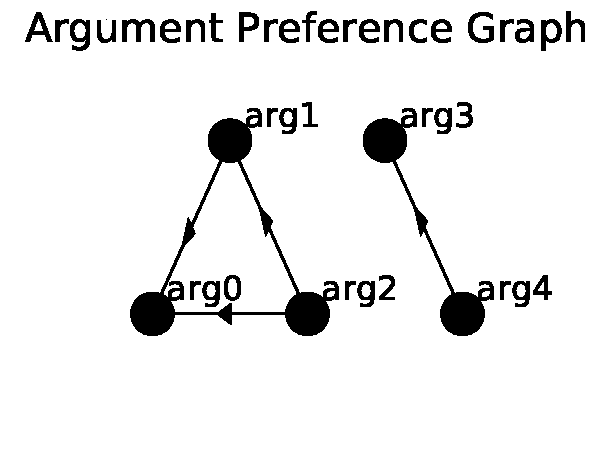
\includegraphics[width=0.5\columnwidth, clip=True, trim=30 30 20 30]{figures/cycles_demo/no_cycle/arggraph_arg_graph}
}
\subfloat[single cycle]{
  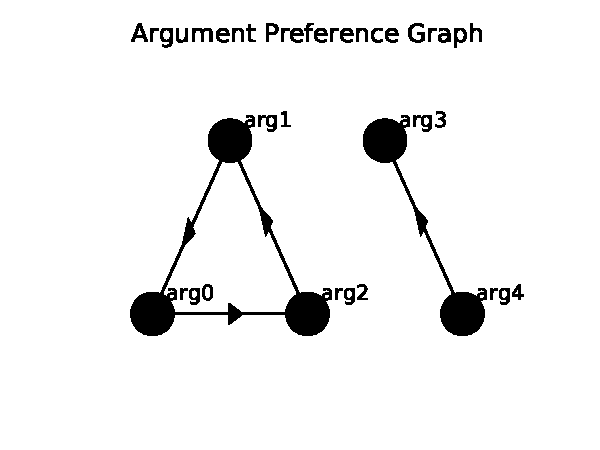
\includegraphics[width=0.5\columnwidth, clip=True, trim=30 30 20 30]{figures/cycles_demo/simple_cycle/arggraph_arg_graph}
}
\subfloat[double cycle]{
  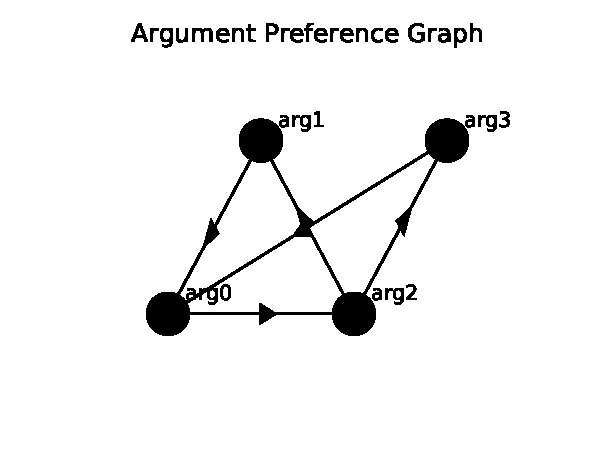
\includegraphics[width=0.5\columnwidth, clip=True, trim=30 30 20 30]{figures/cycles_demo/double_cycle/arggraph_arg_graph}
}
\subfloat[cycle with 9 undecided prefs.]{
  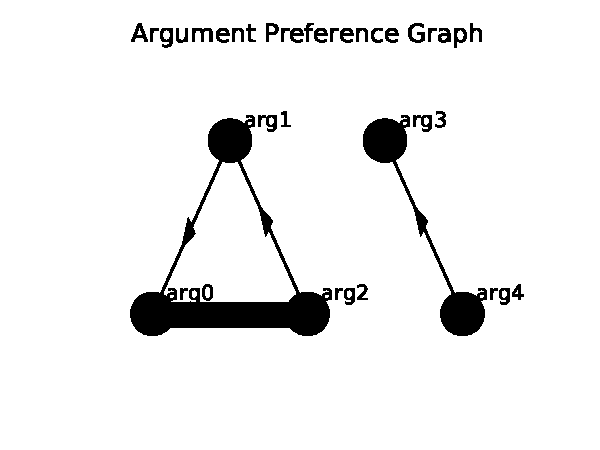
\includegraphics[width=0.5\columnwidth, clip=True, trim=30 30 20 30]{figures/cycles_demo/undecided/arggraph_arg_graph}
}
\caption{Argument preference graphs for each scenario. Arrows point to the preferred argument.}
\label{fig:arg_graph}
\end{figure*}
We test our approach on datasets provided by Habernal and Gurevych~\shortcite{habernal2016argument},
which contain pairwise labels for arguments taken from online discussion forums.
A pairwise label can have a value of $0$, meaning the annotator found the second argument in the pair more convincing,
$1$ if the annotator was undecided, or $2$ if the first argument was more convincing.
To test different scenarios, different pre-processing steps were used to produce the
four datasets shown in Table \ref{tab:expt_data}.
For all datasets we perform 32-fold cross validation, using 31 folds for training and one for testing. 
Each fold corresponds to one of 16 controversial topics, and one of two stances for that topic.
The toy datasets are used to illustrate the different behaviour of our compared methods (described below).
\emph{UKPConvArgStrict} and \emph{UKPConvArgRank} test performance with noise-free labelled data,
while \emph{UKPConvArgCrowdSample} is used to evaluate performance with noisy crowdsourced data 
including conflicts and undecided labels, and to test the suitability of our method for active learning
to address the cold-start problem in new domains with no labelled data.
 
\subsection{Method Comparison}

\begin{figure*}
\centering
\subfloat[no cycle]{
  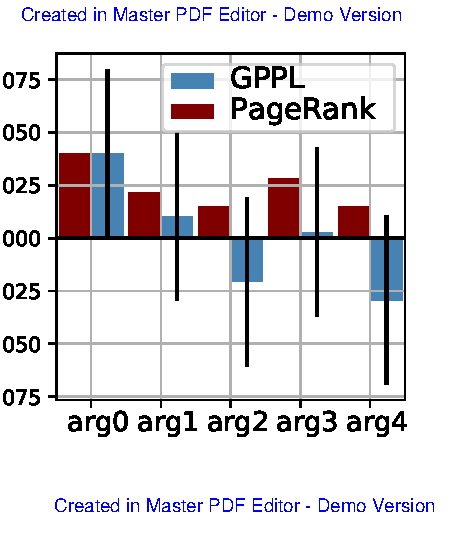
\includegraphics[width=0.4\columnwidth, clip=True, trim=20 5 10 22]{figures/cycles_demo/no_cycle/PageRank_scores}
}
\subfloat[single cycle]{
  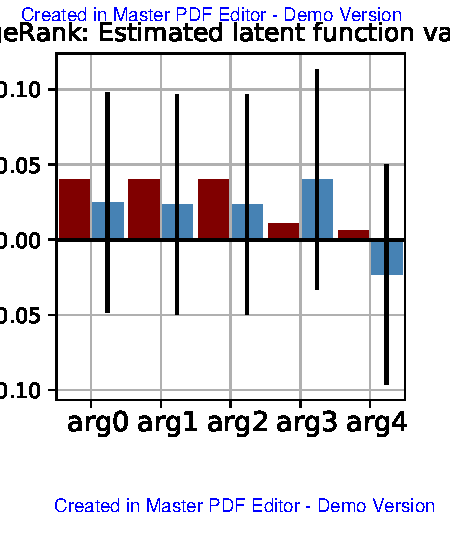
\includegraphics[width=0.4\columnwidth, clip=True, trim=20 5 10 22]{figures/cycles_demo/simple_cycle/PageRank_scores}
}
\subfloat[double cycle]{
  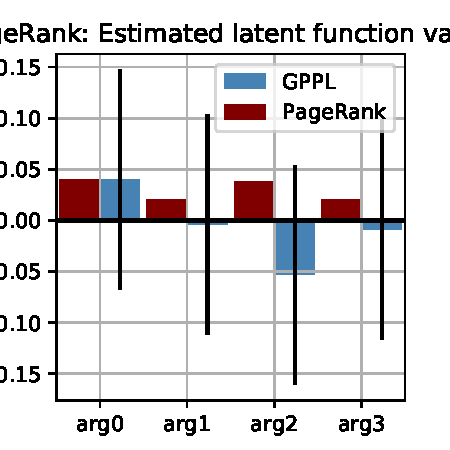
\includegraphics[width=0.4\columnwidth, clip=True, trim=20 5 10 22]{figures/cycles_demo/double_cycle/PageRank_scores}
}
\subfloat[cycle with 9 undecided]{
  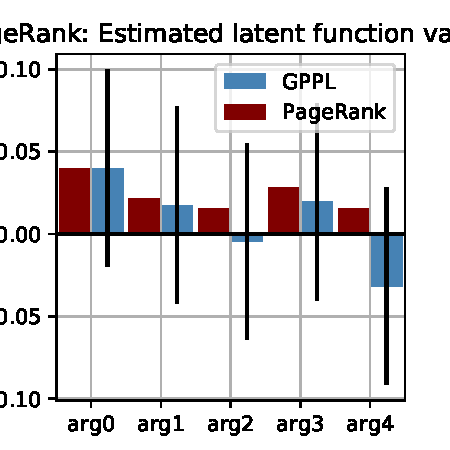
\includegraphics[width=0.4\columnwidth, clip=True, trim=20 5 10 22]{figures/cycles_demo/undecided/PageRank_scores}
}
\caption{Mean scores over 25 repeats. Bars for GPPL show standard deviation of convincingness function posterior.}
\label{fig:scores}
\end{figure*}
Our two basic tasks are \emph{ranking} arguments in terms of convincingness and  
\emph{classification} of pairwise labels for pairs of arguments, i.e. predicting which argument is preferred. 
We compare our scalable Gaussian process preference learning method (\emph{GPPL}) against 
the state-of-the-art SVM approach and a bi-directional long short-term memory network (BiLSTM),
both tested by Habernal and Gurevych~\shortcite{habernal2016argument}.
For both the classification and ranking tasks, GPPL is trained using the pairwise labels for the training folds.
We rank arguments by their expected convincingness, $\mathbb{E}[f(\mathbf{x})]$ for an argument 
with feature vector $\mathbf{x}$, under the approximate posterior $q(f,s)$.
The value of $\mathbb{E}[f(\mathbf{x})]$ is output by our SVI algorithm.
Classification probabilities are obtained by substituting $\mathbb{E}[f(\mathbf{x})]$ for 
$f(v_k)$ or $f(u_k)$ in Equation \ref{eq:pl}.
To apply SVM and BiLSTM to the classification task, we concatenate the feature vectors of each pair of arguments in the training and test sets, and train on the pairwise labels.
For ranking, PageRank is first applied to arguments in the training folds to obtain gold-standard scores from the pairwise labels. SVM and BiLSTM regression models are then trained using the PageRank scores.

As a Bayesian alternative to GPPL, 
we test a Gaussian process classifier (\emph{GPC}) for the classification task 
by concatenating the feature vectors of arguments in the same way as the SVM classifier.
We also evaluate a non-Bayesian approach that uses the same pairwise preference likelihood as GPPL
but trains an SVM regression model instead of a GP (\emph{PL+SVR}).

As input features, SVM uses $\sim32000$ linguistic features, labelled \emph{ling} in the results, 
including unigrams, bigrams, ratios and counts of different parts-of-speech and verb forms,
dependency tree depth, ratio of exclamation or quotation marks, 
counts of several named entity types, POS n-grams,
presence of dependency tree production rules, readability measures,
sentiment scores, spell-checking, and word counts.
BiLSTM uses \emph{Glove} word embeddings with 300 dimensions. Both of these feature sets were
developed by Habernal and Gurevych~\shortcite{habernal2016argument}.

As word embeddings may contain complementary semantic information to linguistic features,
we evaluate GPPL with each feature set and a combination of both, \emph{ling + Glove}.
To create a single embedding vector per argument as input for GPPL,
we take the mean of individual word embeddings for tokens in the argument.
As an alternative,
we also tested skip-thoughts~\cite{kiros2015skip} and Siamese-CBOW~\cite{kenter2016siamesecbow} 
with GPPL on UKPConvArgStrict and UKPConvArgRank, both with ARD optimisation and using the median heuristic,
and alone and combined with \emph{ling}. 
However, we found that mean Glove embeddings produced substantially better performance in all tests.

We set the GPPL hyper-parameters $a_0=2$ and $b_0=200$ after
testing three different settings on UKPConvArgStrict and UKPConvArgRank.
This is a weak prior favouring a moderate level of noise in the pairwise labels.
For the kernel function, $k_d$, we chose the Mat\'ern $\frac{3}{2}$ function due to its 
effectiveness across a wide range of tasks~\cite{rasmussen_gaussian_2006}.
To set the length-scales, we compare the median heuristic (labelled ``medi.")
with MLII optimisation (labelled as ``OptGPPL").

\subsection{Experiment 1: Toy Data}

\begin{figure*}
\centering
\subfloat[no cycle]{
  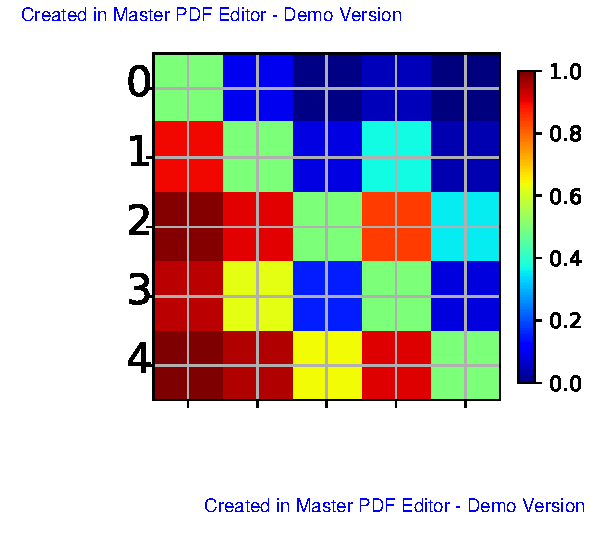
\includegraphics[width=0.36\columnwidth, clip=True, trim=58 5 41 24]{figures/cycles_demo/no_cycle/GPPL_probas}
}
\subfloat[single cycle]{
  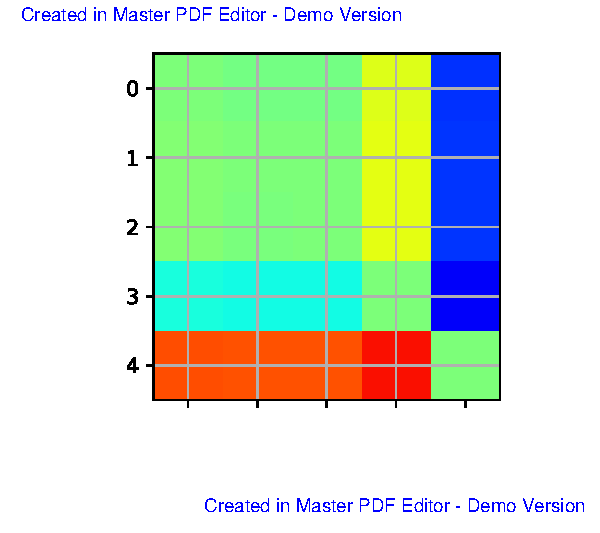
\includegraphics[width=0.36\columnwidth, clip=True, trim=58 5 41 24]{figures/cycles_demo/simple_cycle/GPPL_probas}
}
\subfloat[double cycle]{
  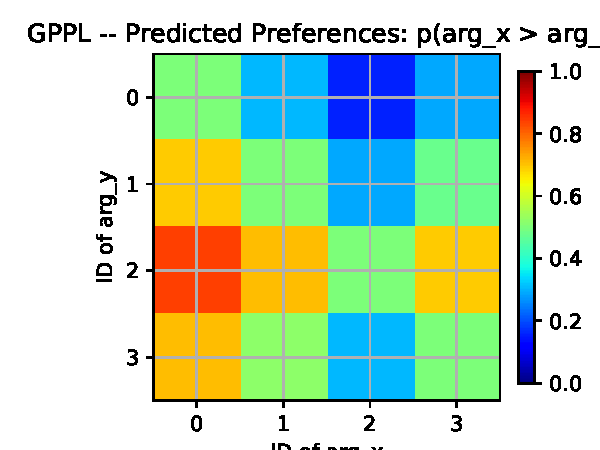
\includegraphics[width=0.36\columnwidth, clip=True, trim=58 5 41 24]{figures/cycles_demo/double_cycle/GPPL_probas}
}
\subfloat[cycle with 9 undecided]{
  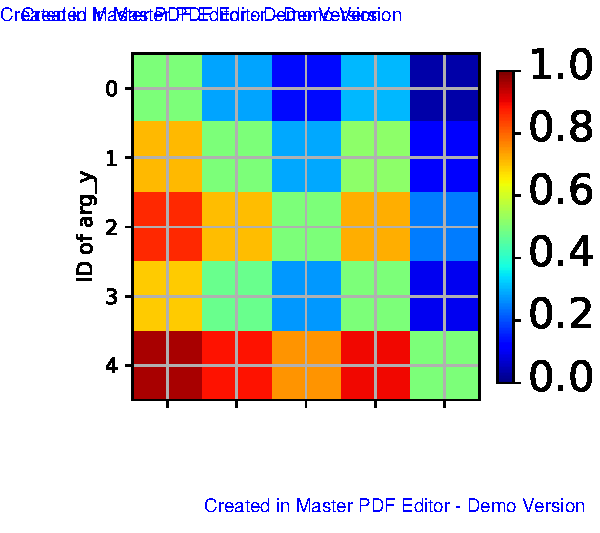
\includegraphics[width=0.42\columnwidth, clip=True, trim=58 5 10 24]{figures/cycles_demo/undecided/GPPL_probas}
}
\caption{Mean GPPL predictions over 25 repeats. Probability that the argument 
on the horizontal axis is preferred to the argument on the vertical axis.}
\label{fig:gppl_classification}
\end{figure*}
\begin{figure*}[t]
\centering
\subfloat[no cycle]{
  \includegraphics[width=0.36\columnwidth, clip=True, trim=58 5 41 24]{figures/cycles_demo/no_cycle/SVM_probas} 
}
\subfloat[single cycle]{
  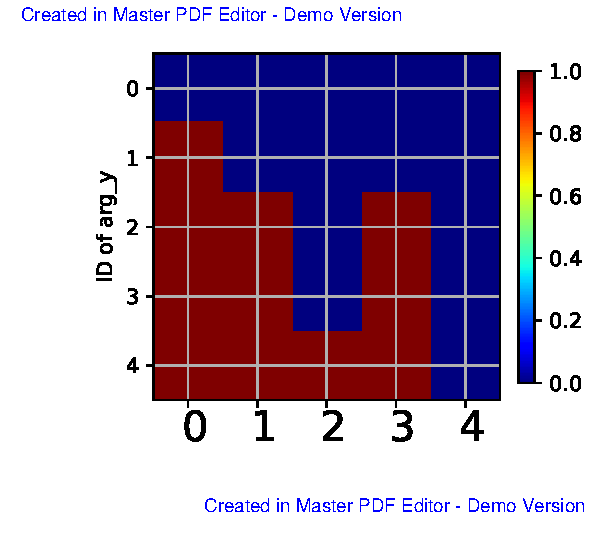
\includegraphics[width=0.36\columnwidth, clip=True, trim=58 5 41 24]{figures/cycles_demo/simple_cycle/SVM_probas} 
}
\subfloat[double cycle]{
  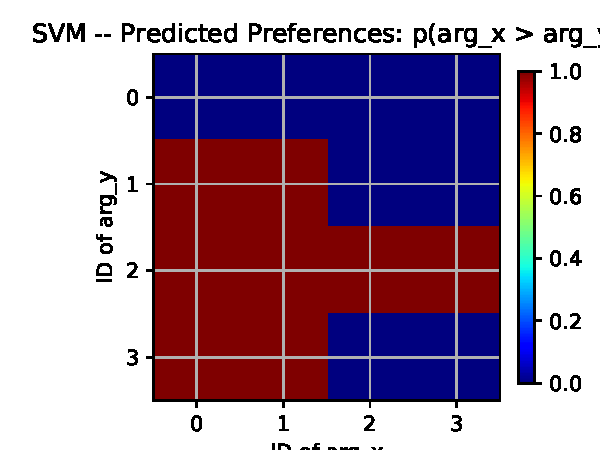
\includegraphics[width=0.36\columnwidth, clip=True, trim=58 5 41 24]{figures/cycles_demo/double_cycle/SVM_probas} 
}
\subfloat[cycle with 9 undecided]{
  \includegraphics[width=0.42\columnwidth, clip=True, trim=58 5 10 24]{figures/cycles_demo/undecided/SVM_probas} 
}
\caption{Mean SVM predictions over 25 repeats. Probability that the argument 
on the horizontal axis is preferred to the argument on the vertical axis.}
\label{fig:svm_classification}
\end{figure*}

We use synthetic data to illustrate the different behaviour of GPPL, SVM for pairwise classification,
and PageRank for scoring arguments.
We simulate four scenarios, each of which contains arguments labelled \emph{arg0} to \emph{arg4}.  
In each scenario, we generate a set of pairwise preference labels according to the 
convincingness graphs shown in Figure \ref{fig:arg_graph}.
Each scenario is repeated 25 times: in each repeat, we select arguments at random from one fold of UKPConvArgStrict
then associate the mean Glove embeddings for these arguments with the labels arg0 to arg4. 
We train GPPL, PageRank and the SVM classifier on the preference pairs shown in each graph and
make predictions for arguments arg0 to arg4.

In the  ``no cycle" scenario, 
arg0 is preferred to both arg1 and arg2, which is reflected in the PageRank and GPPL scores in Figure \ref{fig:scores}. However, arg3 and arg4 are not connected to the rest of the graph and receive different scores with PageRank and GPPL. 
Figure \ref{fig:gppl_classification} shows how GPPL provides probabilistic classifications that are less confident for pairs that were not yet observed, e.g. arg2 $\succ$ arg4. This contrasts with Figure \ref{fig:svm_classification} which shows discrete classifications produced by SVM.

The ``single cycle" scenario shows how each method handles a cycle in the preference graph.
Both PageRank and GPPL produce equal values for the arguments in the cycle (arg0, arg1 and arg2). PageRank assigns lower scores to both arg3 and arg4 than the arguments in the cycle, 
while GPPL more intuitively gives a higher score to arg3, which was preferred to arg4. 
SVM predicts that arg0 and arg1 are preferred over arg3, 
although arg0 and arg1 are in a cycle so there is no reason to prefer arg0 and arg1. 
GPPL, in contrast, gives a weak prediction that arg3 is preferred.

In the ``double cycle" scenario, PageRank and GPPL produce very different results.
Here, the argument graph shows two paths from arg2 to arg0 via arg1 or arg3, and one conflicting
preference arg2 $\succ$ arg0. 
GPPL scores the arguments as if the single conflicting preference, arg2 $\succ$ arg0, 
is less important than the two parallel paths from arg2 to arg0. 
In contrast, PageRank gives high scores to both arg0 and arg2.
The classifications by GPPL and SVM are similar, but GPPL produces more uncertain 
predictions than in the first scenario due to the conflict.

Finally, ``cycle with 9 undecided prefs" shows an exaggerated scenario in which
we have added nine undecided labels to the ``no cycle" scenario, indicated by 
undirected edges in Figure \ref{fig:arg_graph}, to simulate a case where multiple annotators labelled the pair 
and did not all agree. 
This does not affect the PageRank scores, 
but reduces the difference in GPPL scores between arg0 and the other arguments, 
since GPPL gives the edge from arg0 to arg0 less weight due to the undecided labels. 
This is reflected in the GPPL classifications, which are less confident than in the ``no cycle" scenario.
The SVM cannot be trained using the uncertain labels and therefore does not adapt to the undecided labels. 

In conclusion, GPPL appears to resolve conflicts in the preference graphs in a
more intuitive manner than PageRank, which was designed for ranking web pages by 
importance rather than preference. 
In contrast to SVM, GPPL is able to account for undecided labels to soften the latent convincingness function.

\subsection{Experiment 2: UKPConvArgStrict and UKPConvArgRank}

\begin{table*}
\small
  \begin{tabularx}{\textwidth}{ | l  | X |  X |  X |  X |  X | X | X | X |}% X | X |}
  \hline
\multicolumn{9}{| l |}{UKPConvArgStrict} \\   \hline
       &SVM  &BiLSTM&\multicolumn{3}{c|}{GPPL medi.}&GPPLopt. & GPC & PL+ SVR\\\hline
       %& GPPL+, medi. & GPPL+, opt      \\\hline
       &ling &Glove  &ling &Glove &\multicolumn{4}{c|}{ling+ Glove}\\\hline
Acc.:  &0.78 &0.76   &0.78 &0.71  &0.79  & 0.80  & \textbf{0.81} & 0.78\\%& 0.78 & 0.78     \\
AUC:   &0.83 &0.84   &0.85 &0.77  &0.87  & 0.87 & \textbf{0.89} & 0.85\\%& 0.86  &  0.86    \\
CEE:   & 0.52 &0.64  &0.51 &1.12  &0.47  & 0.51 & \textbf{0.43} & 0.51 \\%& 0.69  & 0.69   \\
\hline \multicolumn{9}{| l |}{UKPConvArgRank} \\   \hline
Pearson's r:&0.36&0.32   &0.38 &0.33  & \textbf{0.45} &  0.44 & - & 0.39 \\%& 0.40 &  0.40   \\
Spearman's $\rho$:&0.47&0.37   &0.62 &0.44  &0.65&  \textbf{0.67} & - & 0.63\\% & 0.64 &  0.64   \\
Kendall's $\tau$: &0.34&0.27&0.47 &0.31  &0.49   &  \textbf{0.50} & - & 0.47\\% & 0.49 &  0.49   \\
\hline
  \end{tabularx}
  \caption{Performance comparison on UKPConvArgStrict and UKPConvArgRank datasets. }
  \label{tab:clean_results}
\end{table*}
% \todo{statistical significance? paired Wilcoxon signed-rank test, GPPL ARD vs. SVM. }
% acc p-value of 0.043437
% auc p-value of 0.129870
% cee p-value of 0.000147. 
% Ranking: p-value of 0.000001
% p-value of 0.000001
% p-value of 0.000001
% 
% GPC to GPPL:
% p-value of 0.000012
% p-value of 0.000009
% p-value of 0.000001
% 
% GP+SVR to GPPL:
% p-value of 0.078799
% p-value of 0.056483
% p-value of 0.000171 --> differences mostly not significant
% p-value of 0.085377
% p-value of 0.045415
% p-value of 0.114077
We compare classification performance on UKPConvArgStrict  
and ranking performance on UKPConvArgRank. 
Both datasets were cleaned to remove disagreements between annotators as stated in Table \ref{tab:expt_data}.

The results are shown in Table \ref{tab:clean_results}. When using \emph{ling} features,
GPPL produces similar accuracy and improves the area under the ROC curve (AUC) by 2\%,
and cross entropy error by 0.01.
The AUC quantifies how well the predicted probabilities separate the classes,
while the cross entropy error quantifies the usefulness of the probabilities output by each method.
Much larger improvements can be seen in the ranking metrics. 
When GPPL is run with mean Glove embeddings, it performs worse than
BiLSTM for classification but improves the ranking metrics. Using a combination of features,
GPPL outperforms the alternative methods for both classification and ranking, 
suggesting that embeddings and linguistic features contain complementary information.

Optimising the length-scale using Bayesian model selection improves classification accuracy by 2\% over the median heuristic,
giving a statistically significant improvement over SVM, the previous state-of-the-art ($p=0.0434$ using
two-tailed Wilcoxon signed-rank test).
The differences in ranking metrics between GPPL opt. \emph{ling + Glove}
and SVM are highly statistically significant, with $p <<<0.01$.
However, the cost of these improvements is that each fold required around 2 hours to compute instead of approximately 10 minutes on the same machine (an Intel i7 quad core desktop) using the median heuristic. 

The results show that PL+SVR does not reach the same performance as GPPL, 
suggesting that GPPL benefits from  integrating a GP in a Bayesian manner. 
GPC produces the best results on the classification task, 
indicating the benefits of the Bayesian approach, although it cannot be used to rank the arguments.
The classification improvement over GPPL may result from training directly for this task, 
rather than through a preference learning likelihood. In this experiment, the larger feature space of GPC 
due to concatenating the feature vectors of the first and second items in each pair  
does not seem to have damaged its performance.

\subsection{Experiment 3: Conflicting and Noisy Data}

\begin{table}
\small
  \begin{tabularx}{\columnwidth}{ | l | X | X | X | X | X |}\hline
% \multicolumn{6}{|l|}{UKPConvArgAll} \\   \hline
\multicolumn{6}{| l |}{UKPConvArgCrowdSample} \\   \hline
             & SVM &Bi-LSTM &GPPL medi.        &PL+ SVR     &GPC \\
             &ling &Glove & ling+ Glove &ling+ Glove&ling+ Glove\\\hline
% Acc:     &0.71 &0.73  & 0.77        &0.75       &0.76 \\
% AUC:          &0.81 &0.81  & 0.84        &0.82       &0.86 \\
% CEE:          &0.56 &0.53  & 0.49        &0.52       &0.50 \\
Acc:     &0.70 &0.73  & \textbf{0.77}        &0.75       &0.73 \\
AUC:          &0.81 &0.80  & 0.84        &0.82       & \textbf{0.86} \\
CEE:          &0.58 &0.54  & \textbf{0.50}     &0.55       &0.53 \\
Pears.:      &0.18 &0.26  & \textbf{0.35}        &0.31       & - \\
Spear.:     &0.17 &0.20  & 0.54        & \textbf{0.55}       & - \\
Kend.:      &0.12 &0.13  & \textbf{0.40}        & \textbf{0.40}       & - \\
\hline
  \end{tabularx}
  \caption{Performance comparison on datasets containing conflicts and noise.}
  \label{tab:noisy}
\end{table}
In this experiment, we use UKPConvArgCrowdSample to introduce noisy crowdsourced data 
including conflicting pairwise labels
to both the classification and the regression tasks.
Our hypothesis was that GPPL would be better able to handle unreliable crowdsourced data.

The results in Table \ref{tab:noisy} show that all methods perform worse compared to Experiment 2
due to the noisy pairwise labels. 
GPPL and GPC produce the best results, but GPC no longer has a clear advantage over GPPL. 
GPPL now outperforms the other methods in all metrics except Spearman's $\rho$, where PL+SVR performs slightly better. 
It is possible that GPC and SVM have the
largest drops in accuracy compared to the UKPConvArgStrict results because they 
have no mechanism to resolve conflicts in the preference graph. 
The performance of the BiLSTM classifier also 
decreases by a smaller amount, but was already poorer than the other methods on UKPConvArgStrict. 
PL+SVR is again slightly poorer than GPPL and GPC.
%When noise is introduced in the UKPConvArgCrowdSample dataset, most results drop further. 
% The accuracy of GPC and SVM decreases, as a result of the noise that was introduced,
% while for other methods it remains the same as for UKPConvArgAll. 
Metrics for ranking on UKPConvArgCrowdSample show that while GPPL and PL+SVR continue to perform well, the 
results for BiLSTM and particularly for SVM are much poorer than on UKPConvArgRank. The
differences between GPPL and SVM are highly statistically significant with $p<<<0.01$ for all classification and ranking metrics, as is the difference in accuracy between GPPL and GPC, and between GPPL and PL+SVR.

% \begin{enumerate}
%   \item How much does performance drop when we allow conflicts in the preference graph? Compare GPPL, SVM, Bi-LSTM. Result: all methods have a small drop in performance, but GPPL is affected least.
%   \item How much does performance drop if we use noisy crowdsourced labels, rather than the gold standard produced by MACE? Compare GPPL, SVM, Bi-LSTM. Result: as in previous experiment, GPPL copes best with the added noise. 
% \end{enumerate}
% 
% \todo{statistical significance tests: comparing svm to gppl MH: p-value of 0.000117
% p-value of 0.000030
% p-value of 0.000001
% p-value of 0.000934
% p-value of 0.000001
% p-value of 0.000002. --> ranking is very SS
% GPC to Gppl:
% p-value of 0.001479
% p-value of 0.047469
% p-value of 0.002165 --> ranking difference is SS
% 
% GP+SVR to GPPL:
% p-value of 0.045411
% p-value of 0.082035
% p-value of 0.000012 --> classification is SS but ranking is not
% p-value of 0.088830
% p-value of 0.600577
% p-value of 0.640161
% 
%  }

\subsection{Experiment 4: Active Learning}

In this experiment, we hypothesised that GPPL provides more meaningful confidence estimates than SVM or BiLSTM,
which can be used to facilitate active learning in scenarios where labelled training data is expensive
or initially unavailable.
To test this hypothesis, we simulated an active learning scenario, in which an agent 
iteratively learns a model for each fold. Initially, $N_{inc}=2$ pairs were chosen at random from the training set,
then used to train the classifier. The agent then performs \emph{uncertainty sampling} to select the $N_{inc}=2$
 pairs with the least confident classifications. The labels for these pairs are then taken from the training set and 
used to re-train the model. The result is plotted in Figure \ref{fig:active_learning}, showing that GPPL
is able to reach accuracies above 65\% with only 70 labels, while SVM and BiLSTM do not reach the same performance
given 200 labels. The accuracy of GPPL also increases by approximately 17\% given 200 labels, while SVM increases
approximately 6\% and BiLSTM only 2\%. This suggest that GPPL may be a more suitable model to be used with
uncertainty sampling.
\begin{figure}
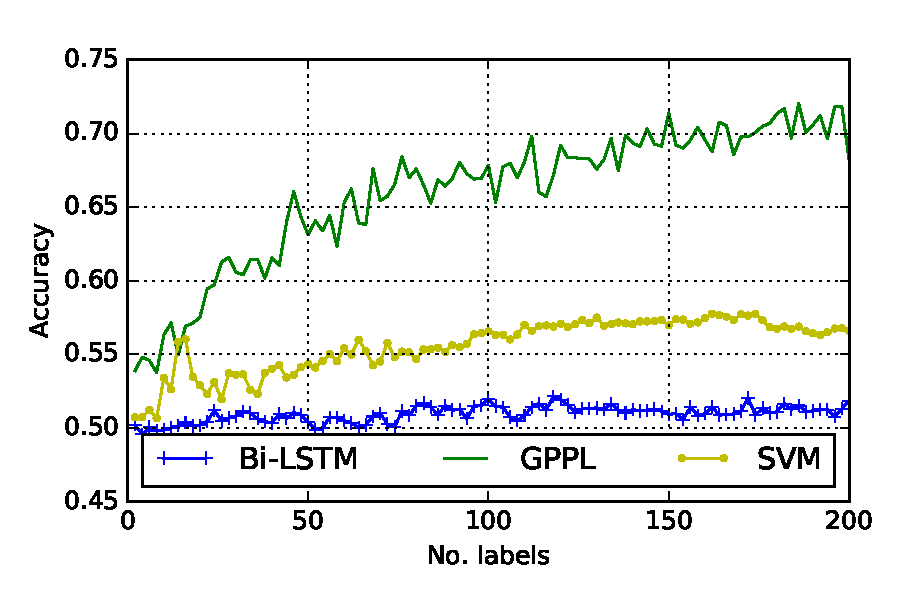
\includegraphics[width=1.0\columnwidth,trim=0 0 0 22,clip=true]{figures/active_learning/test_acc}
\caption{Active learning simulation showing mean accuracy of preference pair classifications over 32 runs.}
\label{fig:active_learning}
\end{figure}

% This plot is invalid because SVM and BiLSTM are trained on the output from PageRank with all the data!
% \begin{figure}
% 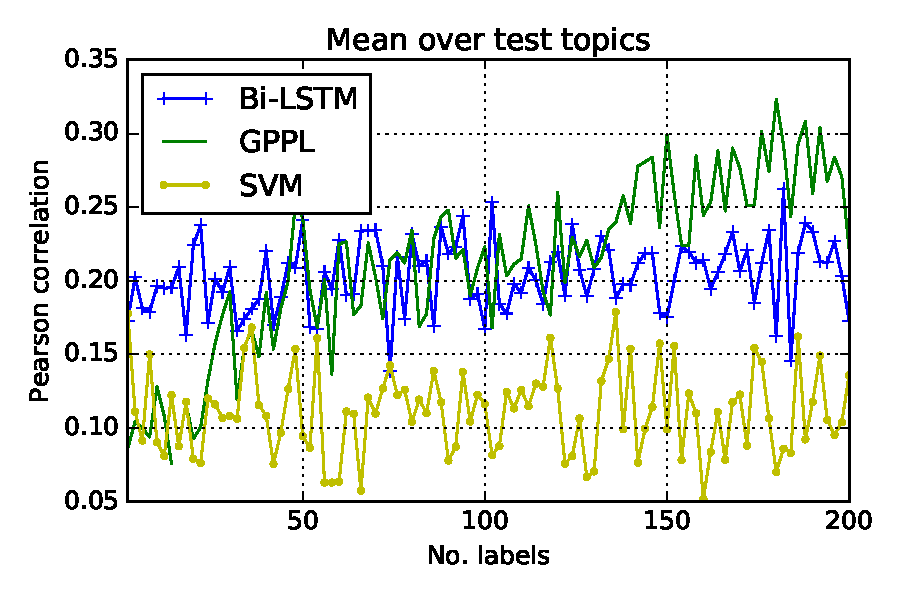
\includegraphics[width=1.0\columnwidth,trim=0 0 0 23,clip=true]{figures/active_learning/test_pearson}
% \caption{Active learning simulation for the three methods showing the mean pearson correlation with the gold standard ranking over 32 runs.}
% \end{figure}

\subsection{Relevant Feature Determination}

% \todo{how much does this really show us? Could we skip this section to make more space for error analysis?
% In contrast with Lampos et al 2014, we cannot identify a small number of important features --> looks like we need
% a combination, perhaps a hierarchical feature representation.}
Finally, we show how the length-scales learned by optimising GPPL can be used to identify
informative sets of features. 
A larger length-scale causes greater smoothing, 
implying that the feature is less relevant when predicting the convincingness function.
than a feature with a small length-scale. 
%In contrast, small length-scales indicate more informative features, since their
%precise value affects the latent preference function.
Figure \ref{fig:boxplot} shows the distribution of normalised length-scales for \emph{ling + Glove}
after optimising on one fold of UKPConvArgStrict. 
Due to the computation time required, our optimisation procedure was limited to $25$ function evaluations,
which may have resulted in the large number of values close to $1$,
% may result from  not being able to optimise all features in the available time.
as features with larger gradients were optimised first.

The length-scales for many dimensions of the mean word embeddings were increased,
giving ratios close to $4$ times the median heuristic, suggesting that these dimensions may be
only very weakly informative. Table \ref{tab:extreme_features} shows the largest
and smallest ratios for embeddings and linguistic features. The unigram "safety" has
a very high length-scale, suggesting it is not informative and may be discarded. 
% It is possible that continuing the optimisation procedure for a larger number of steps would 
% identify large length-scales for other features that may be discarded. However, caution is 
% required to avoid overfitting to the training set during optimisation~\cite{qi2004predictive}.
\begin{figure}[h]
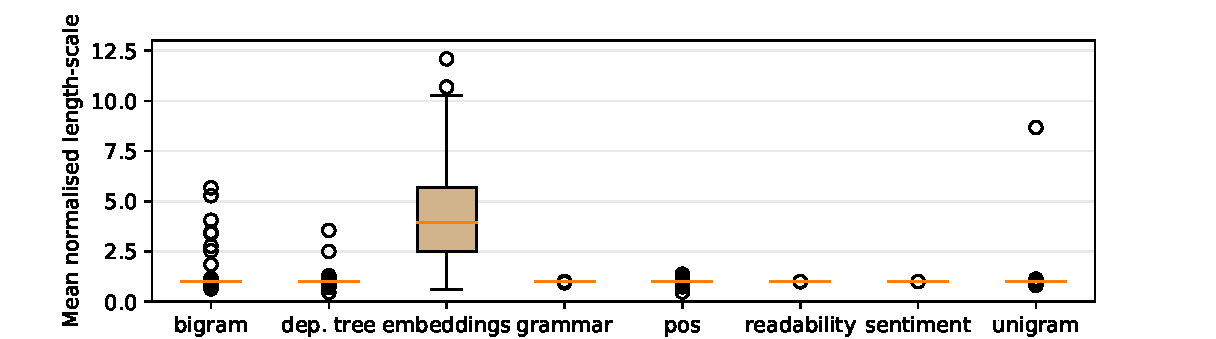
\includegraphics[width=\columnwidth, clip=True, trim=32 0 57 0]{figures/features/boxplot}
\caption{Distribution of length-scales for each type of feature after optimisation. 
Values are relative to the median heuristic value before optimisation, optimised 
on fold "should physical education be mandatory in schools -- no", where 
optimisation increased accuracy from 75\% to 80\%. }
\label{fig:boxplot}
\end{figure}
\begin{table}
\small
  \begin{tabularx}{\columnwidth}{l | X }
  Feature & Ratio\\
  \hline
  ProductionRule-S-$>$ADVP,NP,VP,., & 0.466 \nonumber\\
  Pos-ngram-PP-O-CARD & 0.477 \nonumber\\
  Unigram-``safer", & 0.640 \nonumber\\
  \hline
  Bigram-``?"-``look" & 5.672 \nonumber\\
  Unigram-``safest" & 8.673 \nonumber\\
  Unigram-``safety" & 271.190 \nonumber\\
  \hline
  Embedding-dimension-19 & 0.610 \nonumber\\
  \hline
  Embedding-dimension-241 & 12.093 \nonumber\\
  \end{tabularx}
  \caption{Ratios of optimised to median heuristic length-scales: largest and smallest
  ratios for linguistic features and word embeddings.}
  \label{tab:extreme_features}
\end{table}


\subsection{Error Analysis}

We compared the errors when using GPPL opt. with mean Glove embeddings
and with linguistic features. We
manually inspected the twenty-five arguments most frequently
mis-classified by GPPL \emph{ling} and correctly classified by GPPL \emph{Glove}.
We found that GPPL \emph{ling} mistakenly marked several arguments 
as less convincing when they contained grammar and spelling errors but otherwise
made a logical point. 
In contrast, arguments that did not strongly take a side and did not contain 
language errors were often marked mistakenly as more convincing.

We also examined the twenty-five arguments most frequently misclassified by GPPL \emph{Glove} and correctly labelled by GPPL \emph{ling}.
GPPL \emph{Glove} did not correctly mark arguments as less convincing 
even though they contained multiple exclamation marks and all-caps sentences. 
Other failures were very short arguments and underrating arguments containing the emotive term `rape'.
The analysis confirms that the different feature sets can identify different aspects of convincingness.

% Notes on first paragraph:
% ling failed on:
% overrated: good grammar and structure but weak points?
% both; short and direct argument but not very thoughtful.
% both: seems well structured...
% both: seems to argue for middle ground rather than one side
% both: grammar/spelling errors but strong argument underneath?
% both: grammar/spelling errors but strong argument underneath?
% underrated: very specific example may seem off topic? 
% both: unclear points
% underrated: bad spelling but okay points
% underrated: very personal "I" language to make a good point
% mostly underrated: makes multiple points, some are quite extreme. 
% underrated: sounds quite personal "you" but strong argument.
% both: kind of doesn't try to convince strongly for one side although well written.
%  overrrated: doesn't address the main point although language is reasonable.
% mostly overrated: response to previous answer with no new points.
% underrated: contains '?' and 'you' a lot but makes a good point.
% overrated: language is reasonable, no mistakes, but doesn't clearly take a side.
% overrated: no obvious language indicators but doesn't address main point.
% underrated: lots of spelling mistakes hide the main point.
% mostly overrated: good language but doesn't really support or attack the point directly
% underrated argument with grammatical mistakes but possibly a good point?
% avoiding the argument/debate overrated
% illogical and quite emotional argument underrated
% personal/ad hom attack with 'crap' overrated -- but need to identify the username as such to know it  is a personal attack?
% obvious nonsense without proper words was overrated
%
% embeddings failed on:
%
% both: very short argument, unclear why ling features would help
% overrated: claims lack support
% overrated: spelling mistakes; doesn't address stance of the topic 
% underrated: very short; mean embedding could be an outlier?
% underrated: short
% underrated: no linguistic markers of a bad argument; unclear why embeddings a problem
%     mostly underrated; as above
% underrated: as above; perhaps the words such as 'rape' are associated in the embeddings
% with poor emotional arguments? Perhaps not the word 'rape' itself, but some of the related words in embedding space are common in bad arguments.
% underrated: no idea
% underrated: again mentions 'murder'
% mostly underrated: all caps; why underrated?
% underrated: sensible argument mentions 'personal' a lot
% underrated: very short; mentions wrong and right --> link to emotional arguments without evidence?
% overrated: very short and gives no argument; perhaps contains no bad argument embeddings but linguistic features such as word counts will show it up.
% overrated: mentions of 'dreamt'?
% underrated: no idea
% overrated: doesn't address main point; hard to see why ling would help
% underrated: no idea why; has no linguistic errors
% overrated: no idea; no idea why linguistic features help
% underrated: again maybe because of emotional topic of abortion; no linguistic problems
% overrated: very short sentence; no structure; lots of '!'
% overrated: grammatical errors, very short text that doesn't really make any point or provide any support
% overrated: nonsense detected by all caps
% overrated: very short, cannot really make a good point in that much text
% underrated: why this would beat any other argument is unclear; it's all caps and has lots of '!' too
% 
%  Problem is we don't see what they were misclassified against -- number of 
% misclassifications is too few to know if it is a general problem with that sentence.
% 
% which of these errors are resolved by combining? Pick out errors from either ling that
% were fixed with both; pick our errors from embeddings that were fixed with both.

% when comparing 'both' to 'ling', most of the errors that are made by embeddings
% no longer appear -- those with all caps and '!' have gone. Differences are few.
% seem to be that poorly written arguments continue to be mis-classified.
% with 'both' to embeddings, some of the errors that ling made have gone, e.g. including 'lol'. The remaining ones are mainly those with good superficial structure/correct grammar
% but covering emotional topics. Suggests need for better trade-off between semantics/deeper understanding and linguistic indicators such as good grammar.

% this analysis also shows whether the errors are due to epistemic uncertainty given the features (small difference in 
% similarities between false/true labelled items) or if better training data would help (larger difference between 
% false/true similarities). If GPPL handles the sparse data better, the difference should be reduced compared to SVM.
% the text below is good but the results are not really worth reporting...
%We next investigate whether the Bayesian approach is better able to handle sparsity in the training data. 
%Training data sparsity occurs when the training provides very few examples of arguments in some important regions of feature space, meaning  
% there are arguments in the test dataset that are not similar to any training arguments.
%For each fold, we computed the mean cosine similarity of each argument in the 
%test dataset to the arguments in the training dataset, which we refer to as \emph{training similarity}.
%For UKPConvArgStrict, the mean training similarity for the arguments in pairs correctly classified by GPPL (ling + Glove) was 694.63 and the mean for incorrectly classified arguments was 694.703. This suggests that training similarity is not a strong indicator of a correct
%prediction and training data sparsity does not appear to be a key source of error for GPPL
%in this dataset. In comparison, using  SVM,  
%the mean training similarity for correctly classified arguments
% was 694.72 against 0.     for incorrectly classified arguments, showing that 
% lower training data similarity corresponds to a more misclassified pairs. 
% This indicates that SVM was more affected by training data sparsity.
% However, the small difference in similarities indicates that sparsity was not a problem here?
% The lower similarity of correctly labelled arguments with GPPL suggests it is able to handle more outlying arguments correctly. 
%results: 
% using matern covariance to determine similarity:
% SVM: correctly classified pairs: 694.715334 (STD 3.251511), incorrectly classified pairs: 694.164449 (STD 3.809051). 
% So similarity to training data is higher for correct pairs.
% GPPL: correctly classified pairs: 694.625999 (STD 3.213874), incorrectly classified pairs: 694.703252 (STD 3.580148).
% with cosine similarity:
%SVM For all folds: mean total_sim for correctly classified pairs: 0.998826 (STD 0.021547)
%SVM For all folds: mean total_sim for incorrectly classified pairs: 0.998770 (STD 0.025875)
%GPPL For all folds: mean total_sim for correctly classified pairs: 0.998825 (STD 0.021434)
%GPPL For all folds: mean total_sim for incorrectly classified pairs: 0.998770 (STD 0.026505)
% Using max similarity rather than mean (most similar training point) gives similar results.
% So similarity to training data is actually higher for incorrect pairs; for correct pairs it is lower than for SVM. 
% Suggests that similarity to training data (not being outliers) is less important for GPPL.

To investigate the differences between our best approach, GPPL opt. \emph{ling + Glove}, 
and the previous best performer, SVM, 
we manually examined forty randomly chosen false classifications, where one of 
either  \emph{ling + Glove} or SVM was correct and the other was incorrect. 
We found that both SVM and GPPL falsely classified arguments when they were either very short or long and complex, suggesting deeper semantic or structural understanding of the argument may be required. However, SVM also made mistakes
where the arguments contained few verbs.
%We were not able to identify any common source of error for cases where both 
%methods produced errors. % required deeper semantic understanding and background knowledge of the topics involved
% to evaluate the validity of claims.
% Case 1: SVM right, GPPL wrong.
% underrated, short
% overrated, maybe SVM is right because it dislikes '!'
% underrated, less common language -- perhaps not learned?
% overrated, complex language
% underrated, short argument
% ...
% overrated, irrelevant but well written
% more long arguments with fairly sophisticated language and no obvious errors.
% some cases of arguments that do not take a strong position either way
% The number of errors are small -- could be noise rather than consistent problems with GPPL.
% Some arguments with mainly topic-specific words were misclassified by GPPL but not SVM.
%notable that there are lots of errors on the singapore topics
% Case 2: GPPL right, SVM wrong
% short arguments with few verbs
% long arguments with no obvious language errors and no emotional arguments.
% notable that lots of errors on the school uniform topics

We also compared the rankings produced by GPPL opt. (ling+Glove), 
and SVM on UKPConvArgRank by examining the 20 largest deviations from the 
gold standard rank for each method. Arguments underrated by SVM and not GPPL often 
contained exclamation marks or common spelling errors (likely due to unigram or bigram features).
GPPL underrated short arguments with the ngrams ``I think", ``why?", and
``don't know", which were used as part of a rhetorical question
rather than to state that the author was uncertain or uninformed.
These cases may not be distinguishable using \emph{ling + Glove} features.
% Case 1: GPPL better, SVM worse
% svm underrated some arguments containing !, thankyou, lots of 'if'
% underrated: long argument, common spelling errors (unigrams usually correlated with bad arguments?), India, long and complex arguments, short arguments
% overrated: ('because' could be either over or underrated), mention of another website, 
% Hard to see pattern here because the arguments are very varied in length, grammatical standard; most are not using emotive terms.

% Case 2: SVM better, GPPL worse
% mistakes by GPPL: several short arguments containing "i think"... perhaps leading to a more neutral score than the other features suggest?
% 

% Case 3: GPPL's worst problems (including mistakes by SVM)
% an argument with lots of caps in was underrated
% argument with lots of short sentences (sometimes few verbs) is underrated. 
% underrated: "why?"
% underrated: "don't know" is a big indicator. These two suggest that the model needs a way to determine whether the "don't know" was used in a way that undermines the argument strength (admission of a lack of knowledge) or as a rhetorical device to say that an opposing viewpoint is nonsensical ("don't know why they would do x"). 

% Entropy for SVM correct/incorrect labels: 0.187555, 1.583709
% Entropy for GPPL correct/incorrect labels: 0.128872, 2.443407
% Shows better division between certain and uncertain predictions
An expected advantage of GPPL is that it provides more meaningful uncertainty estimates for tasks such as active learning. 
We examined whether erroneous classifications correspond to more uncertain predictions
when using GPPL and SVM when both methods use the \emph{ling} features.
For UKPConvArgStrict, the mean Shannon entropy
of the pairwise predictions from GPPL 
was 0.129 for correct predictions and 2.443 for errors,
while for SVM, the mean Shannon entropy was  0.188 for correct predictions and 
1.583 for incorrect.
With both methods, more uncertain predictions correlate with more errors,
but the more extreme values for GPPL suggest that its output probabilities more 
accurately reflect the probability of error than those given by the SVM classifier.

% % the analysis below is possible only using the predictions for the training points; however we do not predict for
% % the provided training points?
% To judge whether the GPPL improvements in UKPConvArgCrowdSample are due to better
% handling of noisy labels, we examined whether annotations that disagreed with the 
% MACE gold label -- i.e. erroneous training labels -- led to erroneous predictions. 
% We chart the results of this error analysis in Table \ref{tab:noise_errors}.
% This shows that while arguments with erroneous training labels are more likely to 
% be incorrectly classified using both SVM and GPPL, the Bayesian approach is less susceptible
% to this error.
% \begin{table}
% \begin{tabularx}{\columnwidth}{| l | X | X | X | X | }
% \hline
% & \multicolumn{4}{c | }{\emph{Predictions}} \\
% & \multicolumn{2}{c|}{SVM} & \multicolumn{2}{c|}{GPPL} \\\hline
% \emph{Annotations}           & \emph{True} & \emph{False} & \emph{True} & \emph{False} \\
% Incorrect & & & &  \\
% Correct   & & & & \\
% \hline
% \end{tabularx}
% \caption{Coincidence of erroneous annotations and false predictions by pairwise classification methods.}
% \label{tab:noise_errors}
% \end{table}
